\section{Integración}
\label{sec:integracion}

Para la integración de OpenL Tablets con {\SIDOSPU} existen dos alternativas.

La primera consiste en exponer las reglas por medio de un servicio web utilizando OpenL Rule Services. Esto nos permite integrar con distintas aplicaciones, sobre distintas plataformas, utilizar varias fuentes de datos y exponer varios proyectos y/o módulos mediante un único servicio web.

La segunda alternativa consiste en incluir OpenL Tablets como biblioteca y generar clases wrapper.
Estas últimas se generan en tiempo de ejecución a partir del contenido de las tablas en documentos Excel, exponiendo las reglas definidas en los mismos como métodos.
La principal ventaja de esta opción es que resulta en un menor costo de comunicación, dado que se realiza por medio de llamadas a métodos entre clases Java.

Considerando que las reglas serán utilizadas únicamente por {\SIDOSPU}, y estarán en un único proyecto, no pudiéndose sacar partido de los beneficios de un servicio web, se decidió utilizar la segunda opción.
%
El diagrama en la \cref{fig:integration} muestra un esquema de la integración resultante.
Los rectángulos representan una o varias clases Java, siendo la comunicación entre las mismas por llamado de sus respectivos métodos.

\begin{figure*}
    \centering
    \begin{tikzpicture}[
            auto,
            inner sep=3mm,
            box/.style={draw, rectangle, align=center},
            alt-box/.style={draw, rectangle, align=center, rounded corners=12pt},
            pre/.style={Stealth-},
            post/.style={-Stealth},
            alt-pre/.style={dashed, Stealth-},
            alt-post/.style={dashed, -Stealth},
        ]
        \node[box] (system) {SI-DOSPU};
        \node[box, right=of system] (service) {CalculoReglasServiceImpl}
        edge[pre] (system);
        \node[box, below=0.5cm of service] (clases) {Clases Integración}
        (clases.west) edge[post] (system);
        \node[box, right=of service] (wrapper)  {Clase Wrapper}
        edge[pre] (service)
        edge[post] (clases.east);
        \node[alt-box, above=of wrapper] (rules)  {Reglas (excel)}
        edge[alt-post] node {\small Compilado a} (wrapper)
        (rules.west) edge[alt-pre] node[swap] {\small Lee} (service);
    \end{tikzpicture}
    \caption{Integración OpenL Tablets con SI-DOSPU}
    \label{fig:integration}
\end{figure*}


\subsection{Clases de integración}\label{ssec:integracion:clases}

Como se mencionó en el \cref{sec:motores}, OpenL Tablets permite hacer uso directo de objetos Java dentro de las reglas.
Asimismo, permite hacer uso de clases de forma directa.
Sin embargo, las clases del {\SIDOSPU} lidian con cuestiones no del todo relevantes para el cálculo de las cuotas, como el manejo de errores y el acceso a datos que involucra comunicación con varias clases.
Para evitar contaminar con estos aspectos las reglas de cálculo, se crearon clases que los abstraen:
\begin{itemize}
    \item \scode{Afiliacion} encapsula complejidades de acceder a datos de la afiliación, como la categoría, subcategoría, si tiene cónyuge, etc.;
    \item \scode{Valores}, de manera similar, abstrae el acceso a otros valores del sistema relevantes para el cálculo, como por ejemplo, el \acrshort{cmmu}; y
    \item \scode{Numero}, para poder operar sobre valores de tipo \scode{BigDecimal} utilizando operadores tales como +, -, *, /, etc.
\end{itemize}

\subsection{Formato de las reglas}

OpenL Tablets ofrece una variedad de tipos de tablas \cite{openl}.
Aquí describiremos brevemente el formato de las tablas de decisión, el cual es suficiente para expresar la lógica de negocio del cálculo de la cuota de afiliación.

La tabla de decisión en el \cref{tbl:cambio:original} aborda el caso de los voluntarios adherentes.
El formato de esta tabla, descrito a continuación, es una versión simplificada del formato de las tablas de decisión, pero resulta suficiente para describir las reglas presentadas en este trabajo.

\begin{table*}[h]
    \centering
    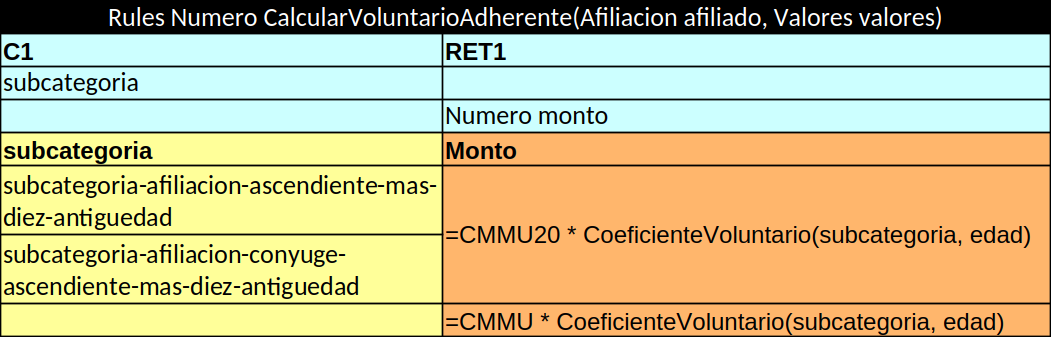
\includegraphics[width=1\textwidth]{voluntario.png}
    \caption{Cálculo de cuota de voluntario adherente}
    \label{tbl:cambio:original}
\end{table*}

La fila 1 contiene el encabezado de la tabla.
En nuestro ejemplo: \tblcode{Rules} indica que la tabla contiene reglas,
\tblcode{Numero} es el tipo de retorno y \tblcode{CalcularVoluntarioAdherente(Afiliacion afiliado, Valores valores)} es el nombre de la tabla con sus dos parámetros.

La fila 2 indica si las columnas forman parte de una condición, indicadas con \tblcode{Cn} para la n-esima condición o retorno \tblcode{RETn} para el n-esimo posible valor de retorno. Las expresiones que son evaluadas en cada condición o retorno se definen en la fila 3. En estas expresiones se puede hacer referencia a los parámetros de la regla, los campos de los mismo y los parámetros definidos en la fila 4. Ésta última especifica el tipo y nombre del parámetro.

La regla del ejemplo cuenta con una condición, que compara la subcategoría del afiliado con un parámetro de nombre \tblcode{valor} y una expresión de retorno vacía, lo que es equivalente a retornar el parámetro de la columna, de nombre \tblcode{monto}.

La fila 5 contiene nombres descriptivos para los parámetros, ignorados por el motor.

Las filas 6, en adelante, especifican los valores concretos para los parámetros.
También pueden contener expresiones matemáticas o llamadas a otras reglas. En estas filas, en las columnas correspondientes a las condiciones, una celda vacía resulta en una condición que evalúa a verdadero.

Para evaluar una regla se evalúan las condiciones utilizando por un lado los valores correspondientes a los parámetros definidos en la fila 1 y por otro los valores de la fila 6, para los parámetros definidos en la fila 4. En caso de evaluar todas las condiciones de a verdadero, se retorna el resultado de evaluar la expresión de retorno. En caso contrario se repite el proceso, pero utilizando los valores de la fila 7 en lugar de la 6. Este proceso continúa hasta todas las condiciones evalúen a verdader o no haya más filas con valores.

Con esto en mente, se puede ver que el ejemplo define una regla de cálculo donde para dos posibles subcategorías se utiliza el valor de referencia \acrshort{cmmu20}, mientras que para todas las demás (dado que se emplea una celda vacía) se la \acrshort{cmmu}. Luego este valor es multiplicado por un coeficiente, que se obtiene llamando a otra regla.

\subsection{Cuota de voluntario jubilado}

El cálculo del monto a abonar por jubilados es uno de los más complejos (junto con el caso de los voluntarios adherentes).
El mismo ocupa más de 150 líneas de código Java en la implementación original del \acrshort{si}.

El cálculo inicia con el \cref{tbl:calculo:jubilado:1}.
Se debe notar un atajo utilizado en la notación para las expresiones de las dos condiciones, \tblcode{C1} y \tblcode{C2}.
Se coloca únicamente, el nombre del campo, que se obtiene del parámetro \tblcode{Afiliado}, cuando la expresión buscada es una igualdad con los valores que se colocarán en las celdas debajo.
Entonces, si el afiliado no tiene haber percibido actualizado, se retorna el valor calculado en el \cref{tbl:calculo:jubilado:sinhaber}. 
En caso de si tenerlo, 
el cálculo continua con el \cref{tbl:calculo:jubilado:sinconyuge} o con el \cref{tbl:calculo:jubilado:conconyuge}, dependiendo de si el afiliado tiene un cónyuge o conviviente que también sea titular en la obra social, o no.

\begin{table*}
    \centering
    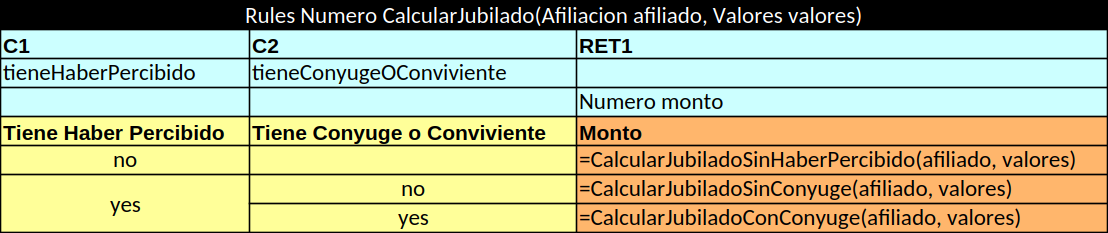
\includegraphics[width=.93\textwidth]{jubilado.png}
    \caption{Cálculo de cuota de jubilado}
    \label{tbl:calculo:jubilado:1}
\end{table*}

El cálculo del monto para un afiliado sin haber actualizado se muestra en el \cref{tbl:calculo:jubilado:sinhaber}.
Se toma como monto la cuota máxima de jubilado por un modificador, el cual se define dependiendo de si tiene un cónyuge o conviviente como afiliado titular.
El caso para voluntario jubilado sin cónyuge titular (responsable de pago) es similar.
El mismo se trata en el \cref{tbl:calculo:jubilado:sinconyuge}.
La diferencia es que se usa la fórmula de cálculo en base a su haber percibido \cref{tbl:calculo:jubilado:base}, en lugar de la cuota máxima de jubilado.

\begin{table*}
    \centering
    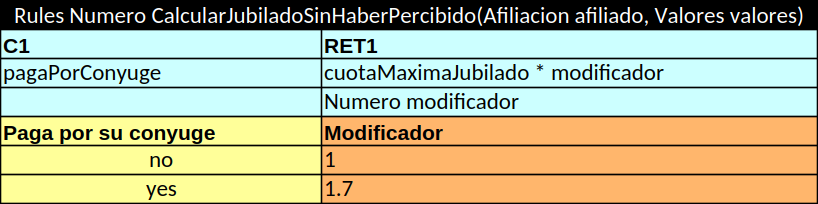
\includegraphics[width=0.70\textwidth]{jubiladoSinHaber.png}
    \caption{Cálculo de cuota de jubilado sin haber actualizado}
    \label{tbl:calculo:jubilado:sinhaber}
\end{table*}


\begin{table*}
    \centering
    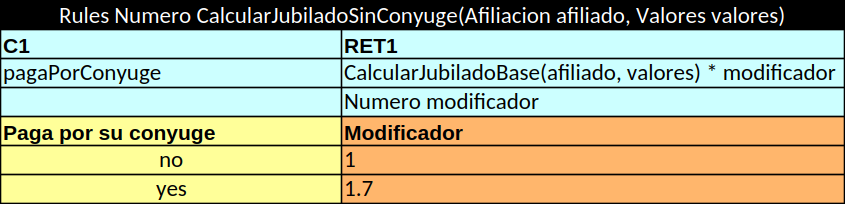
\includegraphics[width=0.71\textwidth]{jubiladoSinConyuge.png}
    \caption{Cálculo de cuota de jubilado sin cónyuge titular}
    \label{tbl:calculo:jubilado:sinconyuge}
\end{table*}

\begin{table*}
    \centering
    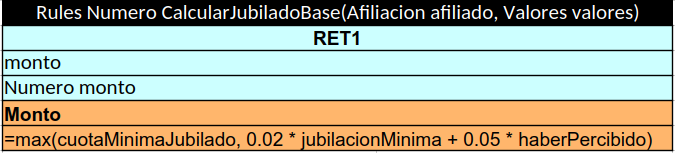
\includegraphics[width=0.63\textwidth]{base.png}
    \caption{Cálculo cuota base jubilado}
    \label{tbl:calculo:jubilado:base}
\end{table*}

El caso de voluntario jubilado con cónyuge titular requiere dos tablas. 
La primera se puede ver en el \cref{tbl:calculo:jubilado:conconyuge}.
En ella se comprueba si su cónyuge es también voluntario jubilado titular.
En caso de serlo, dependiendo de su condición, que debe estar habilitado o en su defecto moroso, y si es responsable de pago y tiene su haber percibido actualizado, se utiliza el \cref{tbl:calculo:jubilado:conyuge:responsable}.
Cabe aclarar que puede ser titular, pero no ser responsable de pago, si su cónyuge pague su cuota. 
En el \cref{tbl:calculo:jubilado:conyuge:responsable} se controla si el voluntario al que se le está cobrando, que tiene cónyuge que también es voluntario jubilado, es el de menor ingresos, para hacer el descuento en el monto.
El tratamiento de este caso puede parecer controlar de manera redundante algunas condiciones. 
Esto es porque el tratamiento de cada afiliado titular se hace de manera independiente, no como grupo familiar.

\begin{table*}
    \centering
    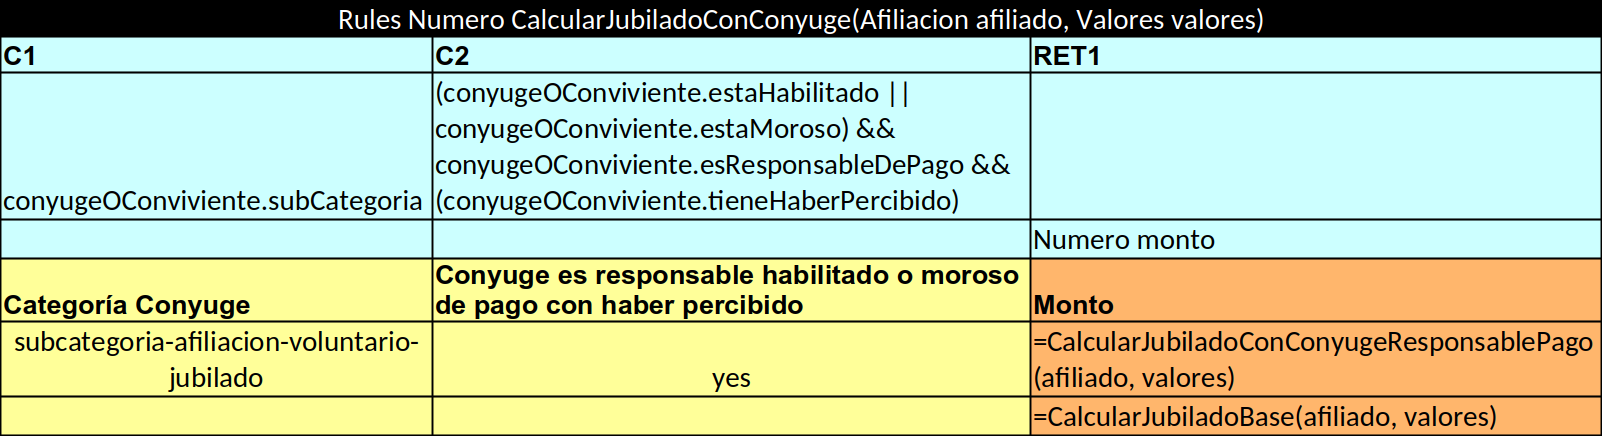
\includegraphics[width=1\textwidth]{jubiladoConConyuge.png}
    \caption{Cálculo de cuota de jubilado con cónyuge}
    \label{tbl:calculo:jubilado:conconyuge}
\end{table*}

\begin{table*}
    \centering
    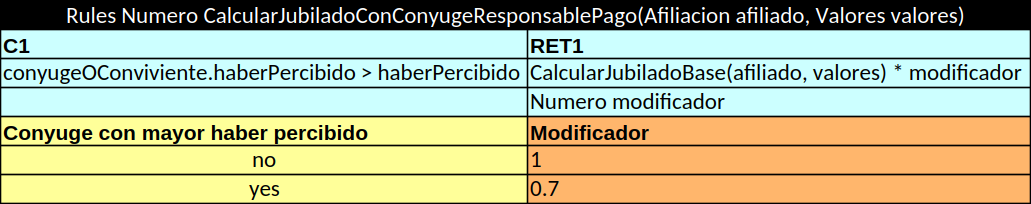
\includegraphics[width=0.85\textwidth]{jubiladoConConyugeResponsable.png}
    \caption{Cálculo cuota jubilado con cónyuge}
    \label{tbl:calculo:jubilado:conyuge:responsable}
\end{table*}

\subsection{Simulando un cambio}
\label{ssec:integracion:cambio}

Para ilustrar las ventajas de integrar el motor de reglas, consideremos la aplicación del siguiente cambio.

\emph{
El cálculo de la cuota de un afiliado agente \acrshort{unsl} con licencia será equivalente al 9\% del sueldo bruto que percibiría si estuviera en actividad. 
De igual forma, dicho monto no puede ser inferior a los porcentajes de la \acrshort{cmmu} que se utilizan en el cálculo anteriormente presentado para la subcategoría.
}

Para implementar el cambio, basta modificar la especificación en el \cref{tbl:cambio:original} para que quede como el \cref{tbl:cambio:cambiado}. 
En este último hay una fila adicional considerando el caso especial introducido para el afiliado agente \acrshort{unsl} con licencia.

\begin{table*}
    \centering
    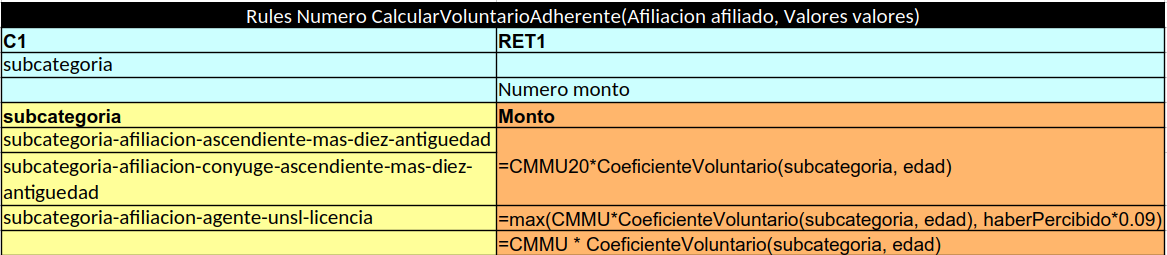
\includegraphics[width=1\textwidth]{voluntario_cambios.png}
    \caption{Cálculo modificado voluntario adherente modificado}
    \label{tbl:cambio:cambiado}
\end{table*}
